\section{Численный метод}
\subsection{Общая идея сеточно-характеристического метода}
\subsubsection{Расщепление по направлениям}

Сведём решение исходной системы в трёхмереном пространстве
\begin{equation}
	\label{matrix_anisotropy_equation1}
	\frac{\partial\vec{u}}{\partial{t}}+\mathbf{A}_x\frac{\partial\vec{u}}{\partial{x}}+
	\mathbf{A}_y\frac{\partial\vec{u}}{\partial{y}}+
	\mathbf{A}_z\frac{\partial\vec{u}}{\partial{z}}=0
\end{equation}
к решению одномерной системы:
\begin{equation}
	\label{norm_form}
	\frac{\partial\vec{u}}{\partial{t}}+\mathbf{A_i}\frac{\partial\vec{u}}{\partial{x_i}} = 0.
\end{equation}

Обозначим оператор $f_i$ как переход с одного временного слоя на другой при численном решении уравнения \eqref{norm_form}:
\begin{equation}
	\label{simple_splitting}
	\vec{u_i}^{n} = f_i(\mathbf{A}_i)\vec{u}^{n},
\end{equation}
а оператор $F$ -- как такой переход для трёхмерного уравнения. Тогда \cite{chelnokov} будет верно с первым порядком точности по времени:
\begin{eqnarray}
\label{simple_3D_split_operator}
F = \alpha_0 f_0(\frac{\mathbf{A}_0}{\alpha_0}) + \alpha_1 f_1(\frac{\mathbf{A}_1}{\alpha_1}) + \alpha_2 f_2(\frac{\mathbf{A}_2}{\alpha_2}), \\
\alpha_0 + \alpha_1 + \alpha_2 = 1,
\end{eqnarray}
и со вторым поряком точности по времени:
\begin{equation}
\label{3D_split_operator}
F = \frac{1}{6}\sum_{i \neq j \neq k \neq i} f_i(\mathbf{A}_i)f_j(\mathbf{A}_j)f_k(\mathbf{A}_k).
\end{equation}

Вычисление по схеме \eqref{3D_split_operator} слишком затратны по количеству вычислений и памяти. Однако, как показывает практика, с достаточной точностью работает следующее к ней приближение:
\begin{equation}
\label{short_3D_split_operator}
F = f_0(\mathbf{A}_0)f_1(\mathbf{A}_1)f_2(\mathbf{A}_2),
\end{equation}
которое является первым слагаемым в \eqref{3D_split_operator}. Такое приближение обладает тем достоинством, что оно не только близко ко второму порядку, но и экономичнее по памяти, чем \eqref{simple_3D_split_operator}.

\subsubsection{Сеточно-характеристический метод в одномерном случае}
Из гиперболичности рассматриваемой системы уравнений следует диагонализуемость матриц $\mathbf{A}_i$:
\begin{equation}
	\label{diagonal_view}
	\mathbf{A} = \mathbf{\Omega}^{-1}\mathbf{\Lambda}\mathbf{\Omega}.
\end{equation}	
Умножим \eqref{norm_form} справа на $\mathbf{\Omega}$:
\begin{equation}
	\label{norm_form1}
	\mathbf{\Omega}\frac{\partial\vec{u}}{\partial{t}}+\mathbf{\Lambda}\mathbf{\Omega}\frac{\partial\vec{u}}{\partial{x}} = 0.
\end{equation}
В приближении локальной однородности среды можно внести $\mathbf{\Omega}$ под знак дифференциала:
\begin{equation}
	\label{norm_form2}
	\frac{\partial(\mathbf{\Omega}\vec{u})}{\partial{t}}+\mathbf{\Lambda}\frac{\partial(\mathbf{\Omega}\vec{u})}{\partial{x}} = 0.
\end{equation}
	
Обозначая $\vec{r} = \mathbf{\Omega}\vec{u},$ получим уравнение:
\begin{equation}
	\label{Riman_invariantes}
	\frac{\partial\vec{r}}{\partial{t}}+\mathbf{\Lambda}\frac{\partial\vec{r}}{\partial{x}} = 0.
\end{equation}
Переходя к производной вдоль направления, заданного уравнением
\begin{equation}
	\label{characteristic_direction}
	\frac{dx}{dt} = \lambda_k, \quad k = \overline{1, 9},
\end{equation}
получим
\begin{equation}
	\label{Riman_invariantes1}
	\left(\frac{dr_k}{dt}\right)_k = 0, \quad k = \overline{1, 9}.
\end{equation}
Отсюда следует, что вдоль этого направления значение $r_k$ сохраняется. Поэтому $r_k$ называются инвариантами Римана, а линии, заданные \eqref{characteristic_direction} -- характеристиками.

В этом и есть суть сеточно-характеристического метода -- перенос значений с предыдущего временного слоя через инварианты Римана.
\begin{figure}[H]
	\center{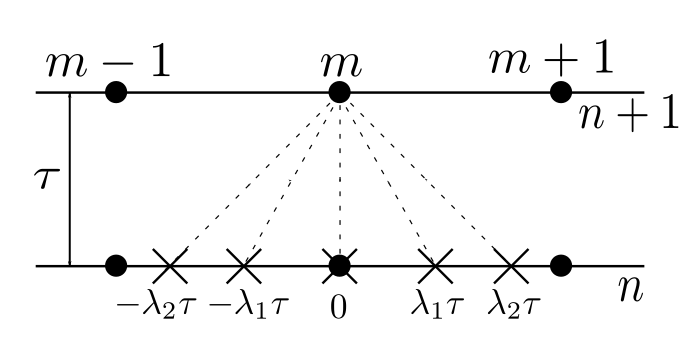
\includegraphics[width=0.5\textwidth]{png/gcm-idea.eps}}
	\caption{Основная идея сеточно-характеристического метода}
	\label{pic:gcm-idea}
\end{figure}
Сформулируем алгоритм одного шага метода по времени (см. \ref{pic:gcm-idea}):
\begin{enumerate}
	\item Из узлов сетки на новом временном слое выпускаются характеристики на предыдущий слой. Количество характеристик равно количеству переменных в системе.
	\item В точках пересечения характеристик с предыдущим слоем вычисляются значения функции и пересчитываются в инварианты Римана.
	\item Инварианты Римана переносятся на новый слой, производится их пересчёт в значения функции.
\end{enumerate}

Описанный выше метод применим только в тех случаях, если точка пересечения выпущенной из расчётного узла характеристики и предыдущего временного слоя не выходит за пределы области интегрирования. Это условие может быть нарушено в нескольких случаях (см. \ref{pic:outer-cases}). Во-первых, в случае граничных узлов, когда направление характеристики вне тела -- точка номер 2. Во-вторых, в случае внутренних узлов, когда характеристика пересекает границу тела до пересечения с предыдущим временным слоем -- точка номер 1. Такая же ситуация возможна и для граничных узлов при наличии острых углов у области интегрирования -- точка номер 3. Рассмотрим каждый из этих случаев по отдельности.
\begin{figure}[H]
	\center{\includegraphics[width=0.8\textwidth]{png/outer-cases.png}}
	\caption{Тело с острым углом на границе. Различные случаи выпадения характеристик за область интегрирования}
	\label{pic:outer-cases}
\end{figure}


\subsubsection{Расчёт граничных узлов}
В \cite{chelnokov} был предложен следующий алгоритм расчёта граничных условий. Сначала вычисления проводятся только для внутренних характеристик -- значения инвариантов Римана, соответствующие выпавшим за пределы области характеристикам, зануляются. Затем применяется граничный корректор, цель которого -- обеспечить выполнение заданных граничных условий.

Запишем общий вид линейного граничного условия:
\begin{equation}
	\label{general_border_condition}
	\mathbf{B} \vec{u} = \vec{b}.
\end{equation}

К примеру, для заданной на границе скорости:
\begin{align}
\mathbf{B} =
\left( \begin{array}{cccccccccccc}
1 & 0 & 0 & 0 & 0 & 0 & 0 & 0 & 0 \\ 
0 & 1 & 0 & 0 & 0 & 0 & 0 & 0 & 0 \\ 
0 & 0 & 1 & 0 & 0 & 0 & 0 & 0 & 0 \\ 
\end{array} \right),
\end{align}

\begin{equation}
	\vec{b} = \left( v_{\xi}, v_{\eta}, v_{\zeta} \right)^T,
\end{equation}
где $ v_{\xi} v_{\eta} v_{\zeta}$ -- компоненты скорости в локальном базисе, связанном с границей тела.

Для заданной на границе внешней силы:
\begin{align}
\mathbf{B} =
\left( \begin{array}{cccccccccccc}
0 & 0 & 0 & n_x & n_y & n_z & 0 & 0 & 0 \\ 
0 & 0 & 0 & 0 & n_x & 0 & n_y & n_z & 0 \\ 
0 & 0 & 0 & 0 & 0 & n_x & 0 & n_y & n_z \\ 
\end{array} \right),
\end{align}
где $\vec{n}$ -- единичная нормаль к поверхности в точке задания условия.

\begin{equation}
	\vec{b} = \left( \sigma_{\xi \zeta}, \sigma_{\eta \zeta}, \sigma_{\zeta \zeta} \right)^T,
\end{equation}
где $\sigma_{\xi \zeta}, \sigma_{\eta \zeta}, \sigma_{\zeta \zeta}$ -- компоненты тензора напряжений в локальном базисе, связанном с границей тела.

Составим из собственных векторов, соответствующих внешним собственным значениям, матрицу $\mathbf{\Omega^{*}}$. Будем искать решение на новом слое $\vec{u}^{n+1},$ удовлетворяющее граничным условиям, в виде
\begin{equation}
	\vec{u}^{n+1} = \vec{u}^{*} + \mathbf{\Omega^{*}} \vec{\alpha},
\end{equation}
где $\alpha$ -- неизвестный пока вектор, $\vec{u}^{*}$ -- решение, полученное на этапе внутреннего расчёта. Тогда для $\vec{\alpha}$ получаем СЛАУ:
\begin{equation}
\label{border_slau}
	\left( \mathbf{B} \mathbf{\Omega*} \right) \vec{\alpha} = \vec{b} -  \mathbf{B} \vec{u}^{*}.
\end{equation}
Такой подход означает вычисление внешних инвариантов Римана из условия выполнения заданных соотношений на границе. Другими словами, мы подбираем линейную комбинацию "пришедших извне"\space{} волн так, чтобы выполнялось граничное условие.
Невырожденность системы \eqref{border_slau} равносильна корректности заданных граничных условий.


\subsubsection{Расчёт внутренних узлов с внешними характеристиками}
Для возможности расчёта случаев, изображённых под номером 1 на рис. \ref{pic:outer-cases}, в \cite{magomedov_kholodov_1988} предложен следующий способ. При выполнении  очередного шага по времени сначала производится расчёт всех граничных узлов. После чего для внутренних узлов с выпавшими за пределы тела характеристиками интерполяция внешних инвариантов Римана производится не по предыдущему временному слою, а по границе тела. Точка, в которой проводится интерполяция, находится между двумя слоями во времени. Такой подход корректен, так как значения на границе на новом временном слое уже посчитаны.

Оставшийся случай под номером 3 мог бы быть выполнен аналогично предыдущему, но при расчёте граничных узлов нельзя проводить интерполяцию во времени, так как нет гарантии, что область интерполяции уже была рассчитана на новом временном слое. Поэтому следует сначала определить значение в точке пересечения характеристики с границей, посчитав в этой точке значение функции как для любого другого граничного узла. Таких "переотражений"\space{} может быть несколько.

Вообще стоит отметить, что сложные случаи при расчёте границы области интегрирования -- определяющая проблема при реализации сеточно\hyp{}характеристического метода на неструктурированных расчётных сетках.



\subsubsection{Расчёт граничных узлов и узлов с внешними характеристиками на структурированной расчётной сетке}
Изложенный выше алгоритм расчёта граничных случаев актуален для неструктурированных расчётных сеток. Для регулярных сеток можно использовать более простой метод фиктивных внешних узлов. Его основная идея -- введение вдоль границ тела вспомогательных расчётных узлов, значения в которых выставляются так, чтобы при сквозном счёте граничных узлов автоматически выполнялись граничные условия. 

Допустим, на границе поставлено условие фиксированной внешней силы
\begin{equation}
	\sigma_{ij} n_j = vec{f}.
\end{equation}
Пусть вдоль рассматриваемой оси граничный узел имеет индекс 0, тогда внутренние узлы имеют положительные индексы, а фиктивные узлы -- отрицательные. Перед очередной ступенью расчёта вдоль данной оси выставим










